% Made up for the tikra gallery: a point on the unit circle, its cosine and its sine. In the
% playground, drag the point around the circle.
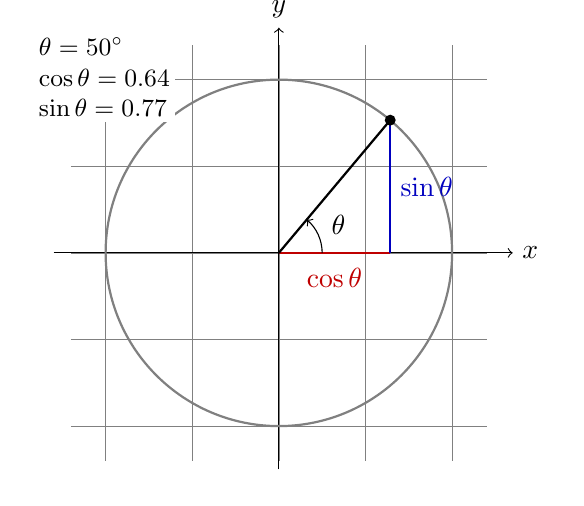
\begin{tikzpicture}[scale=2.2]
  \def\t{50} % angle in degrees, 0..360
  \useasboundingbox (-1.45,-1.3) rectangle (1.6,1.3);
  \draw[help lines, step=0.5] (-1.2,-1.2) grid (1.2,1.2);
  \draw[->] (-1.3,0) -- (1.35,0) node[right] {$x$};
  \draw[->] (0,-1.25) -- (0,1.3) node[above] {$y$};
  \draw[thick, gray] (0,0) circle (1);
  \coordinate (P) at (\t:1);
  \draw[thick, red!75!black] (0,0) -- (P|-0,0) node[midway, below=2pt] {$\cos\theta$};
  \draw[thick, blue!75!black] (P|-0,0) -- (P) node[midway, right] {$\sin\theta$};
  \draw[thick] (0,0) -- (P);
  \draw[->] (0.25,0) arc (0:\t:0.25);
  \node at ({\t/2}:0.38) {$\theta$};
  \fill (P) circle (0.9pt);
  \pgfmathsetmacro\c{cos(\t)}
  \pgfmathsetmacro\s{sin(\t)}
  \node[anchor=north west, font=\small, align=left, fill=white, inner sep=2pt] at (-1.42,1.28) {$\theta = \pgfmathprintnumber[fixed, precision=0]{\t}^\circ$\\
    $\cos\theta = \pgfmathprintnumber[fixed, precision=2]{\c}$\\
    $\sin\theta = \pgfmathprintnumber[fixed, precision=2]{\s}$};
\end{tikzpicture}
